\documentclass[runningheads]{llncs}

\usepackage{graphicx}
\usepackage{todonotes}
\usepackage{listingsutf8}
\usepackage[hidelinks]{hyperref}
\usepackage{cleveref}

\renewcommand\UrlFont{\color{blue}\rmfamily}

\begin{document}

\title{GeoSPARQL 1.1: an almost decadal update to the most important geospatial LOD standard}
\titlerunning{GeoSPARQL 1.1}

\author{
    Nicholas J. Car\inst{1}\orcidID{0000-0002-8742-7730} \and \\
    Timo Homburg\inst{2}\orcidID{0000-0002-9499-5840}\\
%    Simon J.D Cox\inst{3}\orcidID{0000-0002-3884-3420}
}

\authorrunning{Car N.J. et al.}

\institute{
    {
    %SURROUND Australia Pty Ltd., Australia \&\\
    Australian National University, Australia\\
    \email{nicholas.car@surroundaustralia.com}\\
    %\url{https://surroundaustralia.com}
    }
    \and
    {
        Mainz University Of Applied Sciences, Germany\\
        \email{timo.homburg@hs-mainz.de}
    }
    % \and 
    % {
    %     Commonwealth Scientific \& Industrial Research Organisation, Australia\\
    %     \email{simon.cox@csiro.au}
    % }
}

\maketitle

\begin{abstract}
In 2012 the Open Geospatial Consortium published GeoSPARQL 
defining ``SPARQL extension functions'', ``RIF rules'', ``and RDF/OWL ontology for 
[spatial] information'' and supporting vocabularies.\\

In the 8+ years since its publication, GeoSPARQL has become the most important spatial Semantic 
Web standard, as judged by references to it in other Semantic Web standards and its wide use in 
Semantic Web data.\\

An update to the standard was proposed in 2019 to deliver GeoSPARQL 1.1 in 2021 with a charter to: 
handle outstanding change requests and source new ones from the user community and 
to ``better present'' the standard, that is to better link all the standard’s parts and better 
document \& exemplify elements. Expected updates included alignments to other ontologies, 
handling of new spatial referencing systems, new geometry representations, and new artifact 
presentation.\\

In this paper, we will discuss the submitted change requests and resulting updates to the standard. 
We will also discuss the theory behind updates and our expectations for GeoSPARQL 1.1's use.

\keywords{GeoSPARQL  \and GeoSPARQL 1.1 \and spatial \and geospatial \and Semantic Web \and RDF \and OWL \and OGC \and Open Geospatial Consortium \and standard.}
\end{abstract}


\section{Introduction}\label{sec:introduction}
The GeoSPARQL standard, issued in 2012 by the Open Geospatial Consortium (OGC)\footnote{\url{https://www.ogc.org}} 
is one of, if not the most\footnote{It's hard to calculate use but references to GeoSPARQL other well-known standards, 
such as DCAT2 (\url{https://www.w3.org/TR/vocab-dcat/}) suggests this}, used \textit{Sematic Web} standards for 
spatial data.

The original release - GeoSPARQL 1.0 - contained a \textit{specification} document,
a main ``GeoSPARQL'' ontology in an RDF file and a ``Simple Features Vocabulary'' ontology also in an RDF file. The 
``GeoSPARQL'' ontology content, as well as lists of geospatial functions that could be performed on RDF data via 
SPARQL\footnote{\url{https://www.w3.org/TR/sparql11-query/}} queries were defined in the specification document, as
were entailment rules and requirements \& abstract tests for testing ontology data and function implementations. 
Function lists from the specification have been extracted into SKOS\footnote{\url{https://www.w3.org/TR/skos-reference/}}
vocabularies.


\section{Motivation to update GeoSPARQL}\label{sec:motivation}
The OGC \& World Wide Web Consortium's (W3C) \textit{Spatial Data On The Web Working Group}
(SDWWG) established \textit{Spatial Data On The Web Best Practices}\cite{van_den_brink_best_2018} which noted 
shortcomings with then current spatial data standards: ``A best practice for returning geometries in a 
specific requested CRS has not yet emerged''. The group also informally captured specific suggested updates for 
GeoSPARQL\footnote{\url{https://www.w3.org/2015/spatial/wiki/Further_development_of_GeoSPARQL}}, however no updates 
to GeoSPARQL were then made.

Recently, 2019, the OGC reconstituted a \textit{GeoSPARQL Standards Working Group} (SWG) to update GeoSPARQL. The general 
motivation for work within the area of GeoSPARQL, that of \textit{Semantic Web} spatial data, and a series of
fault fixes and proposed extensions to GeoSPARQL 1.0 are captured in an OGC White Paper \cite{geosparqlwhitepaper}. Some,
but not all, of the SDWWG's ideas have been taken up by the SDW, for example the \textit{Best Practices}~\cite{van_den_brink_best_2018}
aspiration that ``A possible way forward is an update for the GeoSPARQL spatial ontology. This would provide an 
agreed spatial ontology, i.e., a bridge or common ground between geographical and non-geographical spatial data...''.
This point has been considered by the SWG and included in future releases' scope. 

Another \textit{Best Practices} issue raised is that ``it makes sense to publish different geometric representations 
of a spatial object that can be used for different purposes''. This is being considered by the SWG with initial
thoughts centering on defining \textit{roles} of geometries with respect to features.

The SWG's charter - its final scope of work - is also published by the OGC \cite{abhayaratna2020ogc} and this guides 
the SWG's activities. Specific actions of the SWG and their staging are explained through the use of a publicly-available 
online task tracking system within the SWG's working online code repository\footnote{\url{https://github.com/opengeospatial/ogc-geosparql/projects/1}}.

At a high-level, proposed updates to GeoSPARQL by both the SDWWG and the SWG may be categorised as one of the following:

\begin{itemize}
    \item[$\ast$] new geometry serializations
    \begin{itemize}
        \item[$-$] GeoJSON, KML itc. Newer, popular format
    \end{itemize} 
    \item[$\ast$] new ontology classes to cater for more nuanced spatial information
    \item[$\ast$] more spatial functions
    \begin{itemize}
        \item[$-$] implementing functions well-known in non \texttt{Semantic Web} spatial systems
    \end{itemize} 
    \item[$\ast$] scalar spatial properties 
    \begin{itemize}
        \item[$-$] area, volume etc. alongside geometries
    \end{itemize} 
    \item[$\ast$] better handling of Spatial (Coordinate) Reference Systems (SRS)
    \begin{itemize}
        \item[$-$] potentially allowing for automated coordinate serialization conversions
    \end{itemize} 
    \item[$\ast$] Internet protocol-based selection of different geometries for features
\end{itemize}

Some of these proposed updates were predicted in GeoSPARQL 1.0, with the \textit{Future Work} section listing several of the 
points above as expected or potential.

The SWG's \textit{Charter}, anticipating that the more obvious updates such as new geometry serializations would certainly
be implemented, listed the following areas of investigation that emerged from SWG proponent's discussions:

\begin{itemize}
    \item[$\ast$] a revision of the ``upper  ontology'' structuring of GeoSPARQL
    \begin{itemize}
        \item[$-$] better/differently defining how GeoSPARQL's \texttt{Feature} and other classes relate to one another and to other fundamental concepts in the ontology
    \end{itemize} 
    \item[$\ast$] alignments to other ontologies, perhaps \textit{W3C Time Ontology in OWL}\cite{simon_cox_time_2017}
    \item[$\ast$] catering for very different SRSes, such as Discrete Global Grid Systems
\end{itemize}

Specifically ruled out of scope was any investigation of property graphs. Recent (last several years) discussion in the OGC and 
elsewhere about property graphs motivated a consideration of them, however, the SWG proponents felt that while property graphs might 
be important for future \textit{Semantic Web} spatial data systems, there was more than enough work scoped for initial SWG work
(several revisions of the standard) to initially exclude this area of investigation.

After initial meetings, the SWG determined to make multiple releases of GeoSPARQL updates with different goals:

\begin{itemize}
    \item[$\ast$] \textbf{1.1}: extensions that are fully compatable with GeoSPARQL 1.0
    \item[$\ast$] \textbf{1.2}: fully or mostly compatable extensions but which are larger additions to the standard's conceptual coverage
    \item[$\ast$] \textbf{2.0}: a future GeoSPARQL that might be quite different and partly incompatable with GeoSPARQL 1.0
\end{itemize} 

The reason for expecting a future, incompatible, GeoSPARQL 2.0 is that early SWG attendees thought spatio-temporal relations
and fundamental ontology elements in GeoSPARQL either could or should be remodelled, which might break the current, familiar, 
\texttt{Feature}/\texttt{Geometry} class relations. Details of these potential changes haven't been fully expounded, at the 
time of this paper, however initial SWG attendees' intuition is that a future GeoSPARQL 2.0 might generalise spatial concepts and
move away from only, or primarily, \textit{geo}spatial, or perhaps focus not just on \texttt{Feature}/\texttt{Geometry} relations
but look to generalised mechanisms for describing dimensions of features of which \textit{geometry} is one of many (and perhaps)
\textit{temporality} too).

An originally unforseen area of updates to GeoSPARQL is new modes of standard presentation. Motivatied by conceptual work within the W3C and the OGC for  
multi-part standards presentation, this has resulted in profile declarations, explained 
in the next section.


\section{Updates in GeoSPARQL 1.1}\label{sec:newfeatures}
So far (as of June, 2020) the GeoSPARQL SWG has triaged change requests for GeoSPARQL releases and has addressed
many 1.1 requests which are the only ons we report here. The next sections foreshadow likely 1.2 and 2.0 updates.

\subsection{Profile Declaration}\label{sec:profiledec}
One of the first actions undertaken by the SWG was to link the GeoSPARQL 1.0 elements through a \textit{profile} 
declaration, where a profile is a special type of \textit{specification}, as defined by \textit{The Profiles Vocabulary}\cite{atkinson_profiles_2020}. 
The specific motivation for this was the SWG's recognition that GeoSPARQL 1.0 consisted of multiple parts, not all
of which were easy to discover. As a result, some GeoSPARQL users were unaware of some of the resources and some
resources were accidentally duplicated or partly re-implemented. Profile declarations of this sort are anticipated, by the OGC, 
as being the \textit{best practice} way for it to deliver multi-part standards.

The profile declaration for GeosPARQL 1.0 will be published by the OGC as a stand-alone resource sometime in early 2021 along with some 
updated GeoSPARQL 1.0 resources. The profile declaration for GeosPARQL 1.1 will be published at the same time as all, or most, of the 
1.1 releases' updated resources, currently expected in mid-2021. The 1.1 releases' resources are:

\begin{enumerate}
    \item a profile declaration
    \item a specification document
    \item an RDF/OWL ontology document
    \item a Functions \& Rules vocabulary, derived from the ontology
    \item a Simple Features feature types vocabulary
    \item a set of RIF\cite{kifer2013rif} rules
    \item SHACL\cite{knublauch_shapes_2017} shapes for RDF data validation 
\end{enumerate}

Both the 1.0 and the 1.1 resources are currently available from the SWG's online code repository\footnote{\url{https://github.com/opengeospatial/ogc-geosparql}}.

\subsection{New geometry literals}\label{sec:newliterals}
Three new geometry serializations are introduced: 

\begin{enumerate}
    \item \textbf{GeoJSON} (Geo- JavaScript Object Notation)\cite{butler2016geojson}
    \item \textbf{KML} (Keyhole Markup Language)\cite{nolan2014keyhole} 
    \item \textbf{DGGS} (Discrete Global Grid System)\cite{sahr1998discrete}
\end{enumerate} 

An example of a point's GeoJSON geometry serialization is given below, followed by an unrelated simple polygon \textit{AusPIX}
\footnote{\url{https://w3id.org/dggs/auspix}} DGGS geometry serialization.

\small
\begin{lstlisting}[caption=GeoJSON geometry serialization example,label=lst:geojsonliteral,language=sql,frame=single,basicstyle=\ttfamily,showstringspaces=false]
"""{"type":"Point", "coordinates":[-83.38,33.95]}"""
^^<http://www.opengis.net/ont/geosparql#geoJSONLiteral>
\end{lstlisting}

\begin{lstlisting}[caption=AusPIX DGGS geometry serialization example,label=lst:geodggsWktliteral,language=sql,frame=single,basicstyle=\ttfamily,showstringspaces=false]
"""<https://w3id.org/dggs/auspix> DirectedOrdinateList 
(R3231 R3234 R3235 R3238 R3243 R3246)"""
^^<http://www.opengis.net/ont/geosparql#dggsWktLiteral>
\end{lstlisting}
\normalsize

GeoJSON \& KML have been much anticipated and were requested by the SDWWG and many users of 
GeoSPARQL, due to those formats' popularity.

The DGGS format is more forward-looking in that it is not driven by user demand but by predicted demand.
DGGS does not have a single, concrete format standard as the others do, nor is it ever likely to - different DGGSes will 
likely implement very different data formats - so GeoSAPRQL 1.1 makes generalized provisions for DGGS serializations but 
presents no detailed requirements for them, only stating that the specific DGGS must be identified.

\subsection{New spatial functions}\label{sec:newfunctions}
While spatial aggregation functions are the norm in many non-semantic geospatial databases such as POSTGIS or Oracle Spatial, 
at the time of defining the GeoSPARQL 1.0 standard, aggregation functions had not yet been introduced into the SPARQL standard,
but have been since with SPARQL 1.1~\cite{w3c_sparql_working_group_sparql_2013}. Spatial aggregation functions 
similar to traditional (relation database), aggregation functions such as AVG, MAX, or MIN allow aggregated results of geometry 
queries, for example, to create the union of a set of selected serialized geometries. While calculating these aggregates is 
certainly possible outside of a semantic database, and thus GeoSPARQL, the inclusion of the functions provides distinct advantages:

\begin{enumerate}
    \item No client-side library is needed to create an aggregated geometry result
    \item Fewer and more appropriate results can be returned using a spatial aggregate function (for example, a union geometry result)
    \item Spatial aggregates from different SPARQL endpoints can easily be calculated using federated queries 
\end{enumerate}

In addition to the \href{http://www.opengis.net/def/function/geosparql/union}{\emph{geof:union}}, \href{http://www.opengis.net/def/function/geosparql/envelope}{\emph{geof:envelope}} and \href{http://www.opengis.net/def/function/geosparql/convexHull}{\emph{geof:convexHull}} functions already defined in GeoSPARQL 1.0, 
for use within SPARQL \texttt{FILTER} operations, GeoSPARQL 1.1 defines \emph{geosf:Union}, \emph{geosf:Envelope} and \emph{geosf:ConvexHull}
as well as \emph{geosf:BoundingCircle}, \emph{geosf:Centroid}, \emph{geosf:ConcatLines} - concatenating a set of overlapping linestrings 
that overlap - and \emph{geosf:ConcaveHull} that can be used to return aggregated results. Listing~\ref{lst:agfunc} gives an example 
of one of these new functions in use.
% \todo[inline]{Timo: I will create a pull request in the GeoSPARQL repository to clear up the issues concerning the spatial aggregate functions. Then I will update the namespaces here. I would find it nice to also include the functions we have discussed yesterday: transformation of SRS and in between literal formats. Should we mention it here as future work or should we make a draft pull request for that so that people have a reference? I think the latter}
\small
\begin{lstlisting}[caption=Aggregation Function example SPARQL query,label=lst:agfunc,language=sql,frame=single,basicstyle=\ttfamily,showstringspaces=false]
# returns the circle geometry bounding all the geometries 
# of Feature <x>
SELECT (geosaf:BoundingCircle(?geo) AS ?circ)
WHERE {
    <x> geo:hasGeometry/geo:asWKT ?geo .
}
\end{lstlisting}
\normalsize

Functions to retrieve min/max values of geometries' coordinates are added: \href{http://www.opengis.net/def/function/geosparql/minX}{\emph{geof:minX}} \& \href{http://www.opengis.net/def/function/geosparql/maxX}{\emph{geof:maxX}},
\href{http://www.opengis.net/def/function/geosparql/minY}{\emph{geof:minY}} \& \href{http://www.opengis.net/def/function/geosparql/maxY}{\emph{geof:maxY}} and \href{http://www.opengis.net/def/function/geosparql/minZ}{\emph{geof:minZ}} \& \href{http://www.opengis.net/def/function/geosparql/maxZ}{\emph{geof:maxZ}}.

\subsection{Ontology extensions}\label{sec:ontexts}
GeoSPARQL 1.1 - see Figure~\ref{fig:geosparql11ontology} for an overview - extends the GeoSPARQL ontology by adding a new class, \href{http://www.opengis.net/ont/geosparql#SpatialMeasure}{\texttt{geo:SpatialMeasure}}. This class represents a spatial measurement 
such as a volume, length, or area associated with a measurement amount and a unit of measure. It is the range of three newly-defined properties:
\href{http://www.opengis.net/ont/geosparql#hasArea}{\texttt{geo:hasArea}}, \href{http://www.opengis.net/ont/geosparql#hasLength}{\texttt{geo:hasLength}} and \href{http://www.opengis.net/ont/geosparql#hasVolume}{\texttt{geo:hasVolume}} which make these attributes of a geometry better accessible using 
SPARQL. 

These additions address a several requests from the SDWWG \& SWG but, given the introduction of a dedicated \textit{measure} class, 
do more too: they open up GeoSPARQL to general patterns of measurement present in ontologies 
such as the W3C's \textit{SOSA}~\cite{haller_semantic_2017}.

The 1.1 release also adds the property \href{http://www.opengis.net/def/function/geosparql/inSRS}{\texttt{geo:inSRS}}, which allows declarations of a geometry's SRS, independent of serializations which paves the way 
for future definition of SRSes in RDF, as anticipated for GeoSPARQL 2.0.

\begin{figure}[htb]
    \centering
    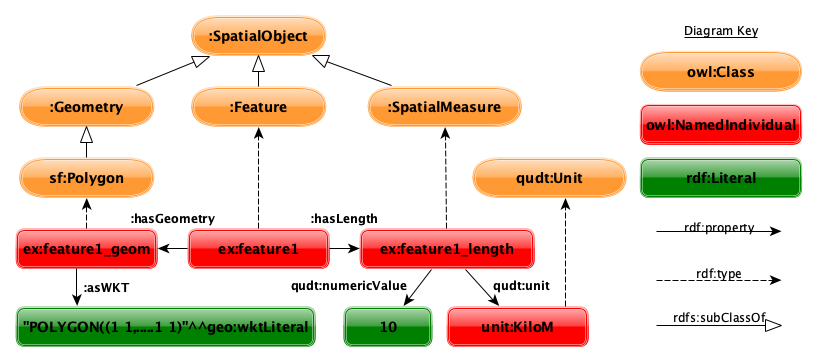
\includegraphics[width=\linewidth]{images/geold_ontology.png}
    \caption{GeoSPARQL 1.1 ontology including one example feature}
    \label{fig:geosparql11ontology}
\end{figure}

\section{Conclusions}\label{sec:conclusions}
A staged schedule of updates to this important \textit{Semantic Web} spatial standard has been initiated with simple and strictly backwards-compatable changes now in GeoSPARQL 1.1. 1.2 will include more detailed work later in 2021 and 2.0, as yet un-specified, might be somewhat different: to be determined by more requirements gathering and feedback on the 1.1 and 1.2 releases.

\subsection{Future Work}\label{sec:futurework}
\begin{itemize}
    \item[$\ast$] GeoSPARQL 1.1: to be completed by July, 2021
    \item[$\ast$] GeoSPARQL 1.2: more adventurous extension - late 2021
    \item[$\ast$] GeoSPARQL 2.0: so-far unspecified
\end{itemize}


%
% ---- Bibliography ----
%
% BibTeX users should specify bibliography style 'splncs04'.
% References will then be sorted and formatted in the correct style.
%
\bibliographystyle{splncs04}
\bibliography{GeoSPARQL}
%
% \begin{thebibliography}{8}
% \bibitem{ref_article1}
% Author, F.: Article title. Journal \textbf{2}(5), 99--110 (2016)

% \bibitem{ref_lncs1}
% Author, F., Author, S.: Title of a proceedings paper. In: Editor,
% F., Editor, S. (eds.) CONFERENCE 2016, LNCS, vol. 9999, pp. 1--13.
% Springer, Heidelberg (2016). \doi{10.10007/1234567890}

% \bibitem{ref_book1}
% Author, F., Author, S., Author, T.: Book title. 2nd edn. Publisher,
% Location (1999)

% \bibitem{ref_proc1}
% Author, A.-B.: Contribution title. In: 9th International Proceedings
% on Proceedings, pp. 1--2. Publisher, Location (2010)

% \bibitem{ref_url1}
% LNCS Homepage, \url{http://www.springer.com/lncs}. Last accessed 4
% Oct 2017
% \end{thebibliography}
\end{document}




% Outline
% 
% Section 1
%   History of GeoSPARWL 1.0
% Section 2
%   motivation to update the spec
% Section 3
%   GeoSPARQL 1.1 additions
%       motivation, and expected use, of new spatial functions. In particular, why in GeoSPARQL when aggregations etc. can be performed elsewhere?
%       Spatial Measure
% Section 4
%       new profile presentation
%       new URI regimes etc
% Section 5
%       expected changed use modes